На рис. \ref{img:frame_lte} изображено формирование кадра в сети LTE. Предположим что мы рассматриваем нисходящее направление соединения и предположим что соединение между UE и eNB уже было установленно. Данные с верхих уровней сначала поступают на PDCP (Packet data compression protocol) уровень. Этот уровень выполняет сжатие и шифрование данных и если необходимо устанавливает проверку на целосность. Далее данные передаются на RLC (LTE Radio Link Control) уровень, который объединяет PDCP PDUs в один RLC PDU.

RLC уровень объединит или сегментирует данные, поступающие от верхнего уровня в правильный размер блока и направит его на уровень МАС со своим собственным заголовком. Теперь MAC уровень выбирает схему модуляции и кодирования настраиваемую на физическом уровне. Эти данные включаются в транспортный блок, который должн быть передан в 1 мс подкадре.

Теперь, рассмотрим количество бит, которые передаются в этом 1 мс интервале. Это зависит от MCS (схемы модуляции и кодирования) и количество ресурсных блоков назначены UE. Мы должны обратиться к таблице 7.1.7.1-1 и таблице 7.1.7.2.1-1 от \cite{3GPPTS36213}.

Давайте предположим, что eNB назначает MCS индекс 20 и 2 блока ресурсов (RB), на основании CQI и другую информацию для передачи по нисходящей линии связи PDSCH (Physical Downlink Control Channel). Тогда необходимо взять значение TBS индекса равным 18, как показано в табл. \ref{TBindex}.

Узнав значение индекса TBS нам нужно обратиться к табл. \ref{TBS}, чтобы найти точный размер транспортного блока (только часть таблицы показан здесь в то время как для полного диапазона значений необходимо обратится к документу \cite{3GPPTS36213}).

Из табл. \ref{TBS} размер транспортного блока равен 776 бит для $I_{TBS}=18$ и  $N_{PRB}=2$. Проще говоря, кодовая скорость может быть определена тем, насколько эффективно данные могут быть переданы в 1 мс транспортном блоке или, другими словами, она представляет собой отношение фактического количества бит передаваемой полезной информации к максимальному количеству бит, которое может передаваться в одном транспортном блоке.


\begin{equation}\label{eq:Reffective}
R_{effective}=\frac{TBS+CRC}{RE \times Q_{m}},
\end{equation}
\noindent где $TBS$ - размер транспортного блока взятый из табл. \ref{TBS}, $CRC$ - циклический избыточный код, $RE$ - ресурсы выделенные или PDSCH или PUSCH, $Q_{m}$ - используемая  схема модуляции, где $\{2,4,6\}$ соответсвуют QPSK, 16QAM и 64QAM.

Пока нам известно $TBS$, $CRC$, $Q_{m}$ и необходимо вычислить $RE$. В нашем случае, предположим, что 10\% $RE$ предназначены для каналов управления (PDCCH и PHICH), то:

$TBS=776$,

$CRC=24$,

$RE=2(RB) \times 12($поднесущих$) \times 7 ($предположим 7 OFDM символа$) \times 2 ($слота на кадр$) \times 0.9 ($ранее предположенные 10\% на управление$)= 302$,

$Q_{m}=6$.

Таким образом $R_{effective}=\frac{776+24}{302 \times 6}=0.4$.

%\clearpage
\begin{figure} [h]
  \center
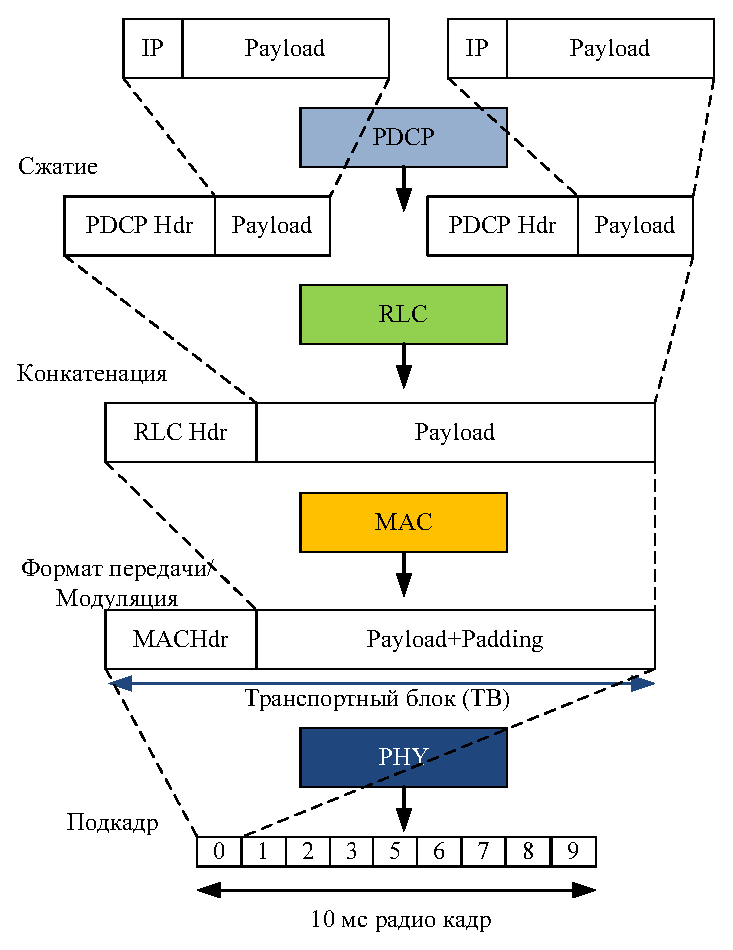
\includegraphics{frame_lte.eps}
  \caption{Формироваие транспортного блока (TB) в LTE}
  \label{img:frame_lte}
\end{figure}



\clearpage

\begin{table} [htb]
  \centering
\parbox{15cm}{\caption{Модуляция и TBS индексы для PDSCH}\label{TBindex}}
    \begin{tabular}{|l|l|l|}
    \hline
     MCS индекс ($I_{MCS}$) &  Порядок модуляции ($Qm$) &  TBS индекс ($I_{TBS}$)    \\ \hline
    0      & 2    & 0         \\ \hline
    1      & 2    & 1         \\ \hline
    2      & 2    & 2         \\ \hline
    3      & 2    & 3         \\ \hline
    4      & 2    & 4         \\ \hline
    5      & 2    & 5         \\ \hline
    6      & 2    & 6         \\ \hline
    7      & 2    & 7         \\ \hline
    8      & 2    & 8         \\ \hline
    9      & 2    & 9         \\ \hline
    10     & 4    & 9         \\ \hline
    11     & 4    & 10        \\ \hline
    12     & 4    & 11        \\ \hline
    13     & 4    & 12        \\ \hline
    14     & 4    & 13        \\ \hline
    15     & 4    & 14        \\ \hline
    16     & 4    & 15        \\ \hline
    17     & 6    & 15        \\ \hline
    18     & 6    & 16        \\ \hline
    19     & 6    & 17        \\ \hline
    20     & 6    & 18        \\ \hline
    21     & 6    & 19        \\ \hline
    22     & 6    & 20        \\ \hline
    23     & 6    & 21        \\ \hline
    24     & 6    & 22        \\ \hline
    25     & 6    & 23        \\ \hline
    26     & 6    & 24        \\ \hline
    27     & 6    & 25        \\ \hline
    28     & 6    & 26        \\ \hline
    29     & 2    &  reserved \\
    30     & 4    & ~         \\
    31     & 6    & ~         \\ \hline
    \end{tabular}
\end{table}



\clearpage

\begin{table} [htb]
  \centering
\parbox{15cm}{\caption{Размеры Транспортных блоков (TBS)}\label{TBS}}
\begin{center}
    \begin{tabular}{|l||l|l|l|l|l|l|l|l|l|l|}
\hline
& \multicolumn{10}{c|}{$N_{PRB}$} \\
\cline{2-11}
\raisebox{1.5ex}[0cm][0cm]{$I_{TBS}$}
& 1   & 2   & 3    & 4    & 5    & 6    & 7    & 8    & 9    & 10   \\
\hline
\hline
    0    & 16  & 32  & 56   & 88   & 120  & 152  & 176  & 208  & 224  & 256  \\ \hline
    1    & 24  & 56  & 88   & 144  & 176  & 208  & 224  & 256  & 328  & 344  \\ \hline
    2    & 32  & 72  & 144  & 176  & 208  & 256  & 296  & 328  & 376  & 424  \\ \hline
    3    & 40  & 104 & 176  & 208  & 256  & 328  & 392  & 440  & 504  & 568  \\ \hline
    4    & 56  & 120 & 208  & 256  & 328  & 408  & 488  & 552  & 632  & 696  \\ \hline
    5    & 72  & 144 & 224  & 328  & 424  & 504  & 600  & 680  & 776  & 872  \\ \hline
    6    & 328 & 176 & 256  & 392  & 504  & 600  & 712  & 808  & 936  & 1032 \\ \hline
    7    & 104 & 224 & 328  & 472  & 584  & 712  & 840  & 968  & 1096 & 1224 \\ \hline
    8    & 120 & 256 & 392  & 536  & 680  & 808  & 968  & 1096 & 1256 & 1384 \\ \hline
    9    & 136 & 296 & 456  & 616  & 776  & 936  & 1096 & 1256 & 1416 & 1544 \\ \hline
    10   & 144 & 328 & 504  & 680  & 872  & 1032 & 1224 & 1384 & 1544 & 1736 \\ \hline
    11   & 176 & 376 & 584  & 776  & 1000 & 1192 & 1384 & 1608 & 1800 & 2024 \\ \hline
    12   & 208 & 440 & 680  & 904  & 1128 & 1352 & 1608 & 1800 & 2024 & 2280 \\ \hline
    13   & 224 & 488 & 744  & 1000 & 1256 & 1544 & 1800 & 2024 & 2280 & 2536 \\ \hline
    14   & 256 & 552 & 840  & 1128 & 1416 & 1736 & 1992 & 2280 & 2600 & 2856 \\ \hline
    15   & 280 & 600 & 904  & 1224 & 1544 & 1800 & 2152 & 2472 & 2728 & 3112 \\ \hline
    16   & 328 & 632 & 968  & 1288 & 1608 & 1928 & 2280 & 2600 & 2984 & 3240 \\ \hline
    17   & 336 & 696 & 1064 & 1416 & 1800 & 2152 & 2536 & 2856 & 3240 & 3624 \\ \hline
    18   & 376 & 776 & 1160 & 1544 & 1992 & 2344 & 2792 & 3112 & 3624 & 4008 \\ \hline
    19   & 408 & 840 & 1288 & 1736 & 2152 & 2600 & 2984 & 3496 & 3880 & 4264 \\ \hline
    20   & 440 & 904 & 1384 & 1864 & 2344 & 2792 & 3240 & 3752 & 4136 & 4584 \\ \hline
    \end{tabular}
\end{center}
\end{table}


